\section{Study 4: Investigating Indirect Conflict Contextual Patterns}
\label{study:apie}

Release points are a vital milestone of software projects. From major releases of a Waterfall based project to iterations of an Agile development,
releases form an interesting single point of a project's development history.
Third party users (outside developers) of a system often only see a product at a release point either major or minor,
and expect the system to come with a sense of reliability and stability at this point. Developers often expect to be able to upgrade a library to
a newer version without having to make major revisions to their own projects to accommodate the upgrade (unless of course patch notes detailing major
changes are released). However, major and minor releases of a library or software resource can cause software quality to degrade in
a third party application as indirect conflicts may occur. The knowledge as to when a project is ready for public usage
as to its reliability, quality, stability, and thus indirect conflict proneness can be a difficult decision to make for most project owners or maintainers.

While measuring software quality has had a major focus in software engineering research for many years~\cite{Bowen:1978:CAS}~\cite{Grady:1993:PRM}~\cite{ISOIEC9126},
the study of software stability and its implications on reliability and indirect conflict proneness remains a difficult subject to understand. 
The decision of what makes a project stable and ready
for a release often comes down to the release manager or maintainer of a project and is often a reflection of the open source community which surrounds 
the project~\cite{Conway:1968}. Code churn is an often looked to statistically for stability but can be grossly misleading
in terms of pre-release and post-release defects~\cite{Fenton:2000:QAF}, with some exceptions~\cite{Nagappan:2005:URC} as well as proneness to indirect conflicts
both internally and externally to third party applications. 
Creating an approach to determining software stability, release preparedness, and the proneness of indirect conflicts is still a large open area of
interest in software engineering research.

In this study, I examine the notions of software change trends, specifically those trends around major releases. Change trends are trends which indicate
a likelihood for a change type to occur around a certain event. Change trends have been used to detect
stability in core architecture~\cite{Wermelinger:2008:AEE} as well as evolving dependencies~\cite{Businge:2010:ESE}.
With the power of major release points in open source projects as a starting point for project stability and the understanding that change trends can
be leveraged to detect stability and the proneness of indirect conflicts, this study investigates the question:

\begin{description}
        \item[RQ\namedlabel{itm:rq1-apie}{RQ1-APIE}] \textit{What trends exist in source code changes surrounding major releases of open 
        source projects as a notion towards a project stability measure?}
\end{description}

In this study, I perform a case study of 10 open source projects in order to study their source code change trends surrounding major release points
throughout their history. I studied 26 change trends quantitatively and 4 change trends qualitatively, and identified a core group of 9 change trends which occur
prominently at major release points of the projects studied. These change trends can provide context as to when indirect conflicts are more likely
to occur based on the findings from Study 3 as I found that indirect conflicts tend to be become less frequent near major release and more
frequent after a release or at the start of a new development cycle. The findings of this study can be applied over the lifetime of a project
to determine the proneness of indirect conflicts and thus aiding developers in dealing with indirect conflicts in their projects.

\subsection{Related Work}
\label{sec:rel}
While very little has been published about release quality studies and stability (especially in regards to
indirect conflicts), there have been a few studies which attempt to address the issues directly
or indirectly. Wu et al.~\cite{Wu:2008:QAF} performed a case study of SoftPM, a widely adopted project management tool, to explore the relationships of
pre-release and post-release failures at major releases. Wu et al. found that the ratio of post-release failures to pre-release failures is significantly low
and can be used to show reliability and stability. Hindle et al.~\cite{Hindle:2007:RPD} performed a case study on MySQL which observed a project's behavior
around major and minor release by monitoring artifact check-ins and changes. They found that there are temporary stoppages for source revisions around releases,
indicating that a temporary freeze is taking place for developers and that last minute fixes and manual testing may be performed.
Zaidman et al.~\cite{Zaidman:2011:SCP}, in comparison, studied the co-evolution of production and test code with inspections and analysis
at major and minor releases, showing how test and production code can evolve at different rates and times. These results show that production
and test code should be handled as different cases for a stability measure around major releases. 

The study of open source projects revolving around release points has become more accessible by the work of Tsay et al~\cite{Tsay:2011:EMO}. Tsay et al. created
a resource of historical release dates for open source software projects to be used for future studies by other researchers.

In terms of software stability, development techniques have been proposed to increase software stability. 
Fayad~\cite{Fayad:2001:TOI}~\cite{Fayad:2002:ASS} suggests that ``business objects'' (BOs) do not change in nature and that they are inherently stable. These
objects only need to change to accommodate external modules at the interface. Some studies such as Chow et al.~\cite{Chow:2011:SJI} have investigated
the stability of changes to interfaces which are considered a good indication of stability.
Mockus et al.~\cite{Mockus:2008:IQR} used major and minor release points to compare industry process quality to customer-perceived quality of the software
project. Mockus et al. found that defect density is lowest at major releases but at the same time software quality is at its lowest all when compared to minor
releases. The low software quality here relates to end-user errors of installations and configurations. Wermelinger et al.~\cite{Wermelinger:2008:AEE}
showed that stable core architectures can be detected by using source code changes. Finally, Fayad et al.~\cite{Fayad:2010:SSM} have
investigated the Software Stability Model (SSM) for Software Product Lines to show that the SSM's impact on architecture and design of a software product
can help improve the life of the product line and make it more adaptable and applicable.

\subsection{Methodology}
\label{sec:apie-meth}
In order to answer my research question, I decided to use the tool ChangeDistiller created by Fluri et al.~\cite{Fluri:2007:CDT}. This tool allows me to detect fine grained
source code changes in Java projects. This tool works by building an abstract syntax tree of a file before and after a code change, then it tries to determine
the smallest possible edit distance between the trees. This results in the source code change at a fine grained level performed in the commit.

I conducted a case study of 10 open source Java projects. These projects are: eclipse.jdt.core, eclipse.jdt.ui, eclipse.jetty.project, 
eclipse.mylyn.commons, eclipse.mylyn.context, hibernate-orm, hibernate-ogm, hibernate-search, eclipse.maven.core, and eclipse.maven.surefire. These project were chosen
because ChangeDistiller only works for Java source code and because of their high use amongst other Java projects and to study specific ecosystems 
of projects and their evolution trends.

For each of the projects, I obtained the software configuration management (SCM) system
which is used to store all source code changes of a project. When it was necessary, I converted some forms of SCM system to Git in order to reduce implementation
burdens of using multiple SCMs. Once the SCM was obtained, I used ChangeDistiller and iterated over every commit found in a project's git master branch. I stored
34 of ChangeDistiller's built in source code change types for each commit. I noted how many of each change type was performed in each commit and stored that information
in a PostgreSQL database. In order to filter and protect my results, I manually inspected the 10 Java projects studied in order to identify code built for test
purposes.
I separated changes to this test code from all other code to ensure my results only focused on real implementation while allowing us to study changes to
test based code separately.

Once the ChangeDistiller information was collected, I decided to examine software change trends surrounding releases of the projects I had selected. Since releases
have preconceived notions of software stability and a lack of proneness to indirect conflicts, 
I decided that by studying the change types surrounding these releases, I could get a better understanding of
what types of source code changes or trends constitute software stability or maturity. In order to study the release points, I went to each of my 10 project's 
web pages and looked through their release histories for major, minor, alpha, beta, and release candidate type releases. In total I identified 472 releases
across my 10 studied projects.  

Once the release dates were collected, I set about analyzing my data by creating average change ratios surrounding the release dates of each 
project as a way to measure the trend of a particular change type at a release type. This change ratio simply compares the number of change events (of a given
change type) before a release to after the release. Both of the before and after event totals are divided by the number of commits on their respective side
of the release to account for activity. I implemented this algorithm through Equation~\ref{eq:norm}.

Equation~\ref{eq:norm} works to create a change ratio by first creating a numerator by summing across all releases of
a given release type a sum of a particular change type in commits ($T_c$)
from the release date ($r$) to a given number of days after the release ($d$) divided by the number of commits in this date range ($|c|$). Next the denominator
is created by summing across all release of a given release type
a sum of that same particular change type in commits ($T_c$) from a given number of days ($d$) before the release date ($r$) to
the release date divided by the number of commits in this date range ($|c|$). This numerator and denominator form the final change ratio.
This equation gives us a ratio of a particular change type happening before and after a particular release. If the ratio is above 1 then that particular change
type occurs more frequently after the release and if it is below 1 then it occurs more frequently before the release. For the purposes of my study, I set the
number of days before and after the release ($d$) to 60 as the projects studies had many months in between their major releases. This quantitative data
formed much of the basis for the results to come in Section~\ref{sec:apie-results}

\begin{equation}
\text{ChangeRatio} = \frac{ \sum_{r_0}^{r_n}\sum_{c=r}^{r+d} T_c / |c|} { \sum_{r_0}\sum_{c=r}^{r-d} T_c / |c|}
\label{eq:norm}
\end{equation}

Aside from generating quantitative data, I also created a web application for the visualization of the data called API Evolution (APIE). This visualizer allowed
me to inspect a single project and a single change type metric at a time (see Figure~\ref{fig:apie}) for qualitative analysis of software evolution trends. I
used this tool to manually inspect 4 specific change type trends surround release dates. To do this, I aggregated change types across 50 commits, meaning that
each point in the graph represented the date of a commit and the sum of the particular change type's occurrences over the last 50 commits. This was used to smooth
out the curves presented by the tool to allow easier manual inspection. This method however does not take activity into account as seen in
Equation~\ref{eq:norm}, so it represents the true activity and change types occurring. Manual inspections were labeled into 4 categories: upward trending, local maximum, downward
trending, and local minimum. Since the graphs were quite turbulent, best estimations were conducted by two judges at each release point to fit the graph into the aforementioned
4 slope categories. The two judges used 1.5 months before and after the release date as start and end points for the graph trend line.

% APIE graph figure
\begin{figure}[tb!]
\centering
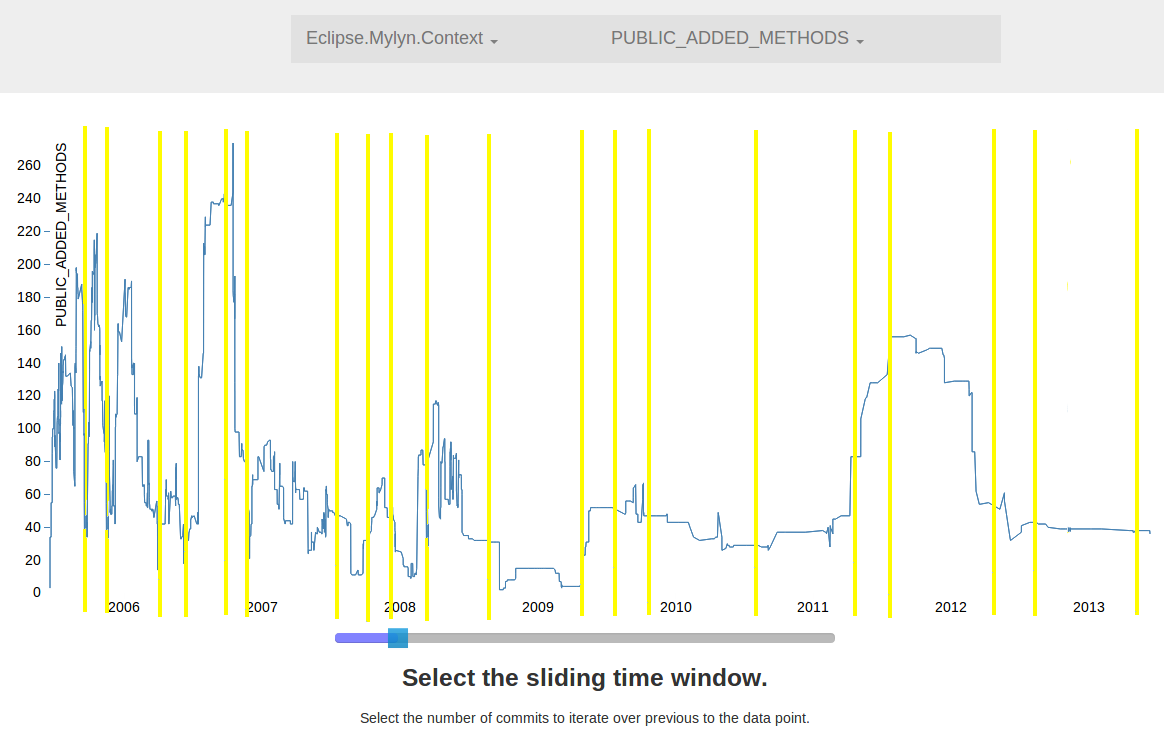
\includegraphics[width=0.9\textwidth]{figures/APIE.png}
\caption{A screen shot of the APIE visualizer showing project Eclipse.Mylyn.Context with change type PUBLIC\_ADDED\_METHODS being analyzed and showing
major releases as vertical yellow lines.\label{fig:apie}}
\end{figure}

I performed 1888 manual inspections across 10 projects, 472 release dates and 4 change types, and used this data to form the basis of my qualitative data.
Quantitative data was used to compliment the quantitative ratios found from the previous methodology. 

\subsection{Results}
\label{sec:apie-results}

Due to time requirements, I focus my results on major releases of the 10 case study projects and select few of the calculated change ratios. 
There were 109 major releases across the 10 studied projects. All of the major findings as per values computed from Equation~\ref{eq:norm} for non test metrics
can be seen in Table~\ref{tab:apie-ratio}.

\begin{table}[ht]
\begin{center}
\tabcolsep=0.11cm
\begin{tabular}{| l | c | c | c |}
\hline
Object & Added & Changed & Removed\\
\hline
Public Classes & 1.14 & 0.86 & 1.16 \\
Public Methods (Signature) & 1.07 & 0.92 & 1.34 \\
Public Methods (Bodies) & - & 1.06 & - \\
Private Classes & 0.81 & 1.18 & 1.44 \\
Private Methods (Signatures) & 1.00 & 1.10 & 1.22 \\
Private Methods (Bodies) & - & 1.08 & - \\
Files & 1.12 & 0.96 & 1.14 \\
Documentation & - & 0.99 & - \\
\hline
\end{tabular}
\end{center}
\caption{Implementation oriented change types and their normalized average change ratios at 60 days on each side of releases. \label{tab:apie-ratio}}
\end{table}

To study the most prevalent change trends, I set a ratio threshold of greater than 1.2, or less than 0.83 (20\% greater trend of after the release date
or 20\% greater trend of before the release date) to indicate the greatest trends.

I found 9 major change trends which surround major releases in the open source
projects studied. 4 change trends found that occur before major releases are: added private classes, 
changed test method signatures, changed documentation, and removed test classes.
5 change trends found that occur after major release are: added test methods, changed test classes, removed public methods, removed
private classes, and removed private methods.

As it can be seen in Table~\ref{tab:apie-ratio}, there are few change type trends around major releases which pass my threshold. We can see that both public
and private methods
being removed from a project is more likely to occur after a major release than before. Table~\ref{tab:apie-ratio} also shows significance in the changes to private
classes. We see that private classes are added more (24\%) before a major release and removed more after (44\%) the release. 
All results in Table~\ref{tab:apie-ratio} could be used as identified trends of major software releases, while I have just highlighted the larger ratios
which meet my threshold criteria.

Another interesting trend that can been seen in Table~\ref{tab:apie-ratio} is that of changes to public objects. We can see for public classes and methods that
5 out of 7 ratios indicate changes occur to these objects after major release rather than before. I hypothesize that these changes to the public API
after a major release come from newly reported bugs from end users as well as having old features being deprecated while adding new features to the project
after the stable build had been released.

My complementary qualitative results from manual graph inspections can be seen in Table~\ref{tab:qual}. These results show that adding, changing signatures
and bodies of, and removing public methods tend to all be at a local minimum of change type trends at major releases when activity is not taken into
account. These results confirm previous results of low code churn as an indication of stability.

\begin{table*}[ht]
\begin{center}
\begin{tabular}{| p{2cm} | c | c | c | c |}
\hline
Change Type & Upward Trend & Local Maximum & Downward Trend & Local Minimum\\
\hline
Added Public Methods & 21.6\% & 17.2\% & 14.7\% & 33.6\% \\ \hline
Changed Public Methods (Signature) & 6.0\% & 19.8\% & 19.0\% & 39.7\% \\ \hline
Changed Public Methods (Bodies) & 9.2\% & 16.5\% & 26.6\% & 37.6\% \\ \hline
Removed Public Methods & 7.8\% & 16.4\% & 12.9\% & 41.4\% \\ \hline
\end{tabular}
\end{center}
\caption{Qualitative graph analysis results. \label{tab:qual}}
\end{table*}

Lastly, I found that software changes related to testing can be an indicator of a major release points within the projects studied. The change
ratios found can be seen in Table~\ref{tab:test}. As it can be seen, the four ratios which meet my threshold and are indicators of stability with regards to test based
changes are: the changing of test classes, the removal of test classes, the adding of methods, and the changing of method signatures, and test classes being changed.
Changes to documentation also meets my threshold and occurs more before a major release.

\begin{table}[ht]
\begin{center}
\begin{tabular}{| l | c | c | c |}
\hline
Object & Added & Changed & Removed\\
\hline
Classes & 1.07 & 1.21 & 0.76 \\
Methods (Signatures) & 1.23 & 0.83 & 1.01 \\
Methods (Bodies) & - & 0.90 & - \\
Documentation & - & 0.72 & - \\
\hline
\end{tabular}
\end{center}
\caption{Test oriented change types and their normalized average change ratios at 60 days on each side of releases. \label{tab:test}}
\end{table}

While all change ratios may need to be considered for continued analysis or a taxonomy of change trends, I have offered the strongest
change trends in these results as a suggestion for future focus.

\subsection{Conclusions of Study}

In this study, I have conducted a case study of 10 open source Java software projects in order to study their change trends surrounding
major releases as previous studies have shown that indirect conflicts occur less at a major release and more so after a major release
or at the beginning of a development cycle. I have presented here 9 major change trends which surround major releases in the open source
projects studied. The 4 change trends found in this study occurring before major releases are: added private classes, 
changed test method signatures, changed documentation, and removed test classes.
The 5 change trends found in this study occurring after major release are: added test methods, changed test classes, removed public methods, removed
private classes, and removed private methods.

These 9 change trends can be used in future indirect conflict tools in order to identify a context for indirect conflicts.
For example. Any of the 9 change trends which occur more so after a major release may be used as a sign of high indirect conflict proneness
since after a major release a new development cycle is likely to begin. As per change trends which occur more so before a major release, indirect
conflict tools may use this context in order to identify a low proneness to indirect conflicts in their results. These two contextual patterns
can be used throughout the life of a software project in order to help better inform indirect conflict tools as to the processes of developers
and provide better feedback to said developers of indirect conflicts.

Aside from contextual patterns for indirect conflicts, this study has also shown the beginnings of a visualization for source code change trends which may
be used as a visual cue towards project stability and potential areas of instability where action may need to be taken.